
\section{模型准备}
\label{sec:preliminary}
本节简要介绍自组织映射神经网络(SOM)以及相关知识.

\subsection{模型符号说明}

\begin{table}[h]
	\begin{center}
		\caption{SOM模型相关符号说明}
		\begin{tabular}{l|c}
			\toprule[2pt] 
			    符号 & 意义 \\ \hline
			 $X_i$& 样本结点\\
       $W_j$&神经元结点\\
       $n$&迭代步数\\
       $\sigma$&邻域半径\\


			\toprule[2pt] 
		\end{tabular}
		
		\label{tab:distribution}
		\vspace{-0.4cm}
	\end{center}
\end{table}


\subsection{自组织映射神经网络}
\label{sec:som}
自组织映射神经网络(Self-Organizing Map, SOM)或自组织特征映射(Self-Organizing Features Map, SOFM)是一种无监督的人工神经网络, 于1982年被Kohonen提出\cite{som}. 不同于一般神经网络基于损失函数的反向传递误差来训练, 它运用竞争学习(competitive learning)策略, 依靠神经元之间互相竞争逐步优化网络,且使用近邻关系函数(neighborhood function)来维持输入空间的拓扑结构.

\begin{figure}[h]
    \begin{center}
        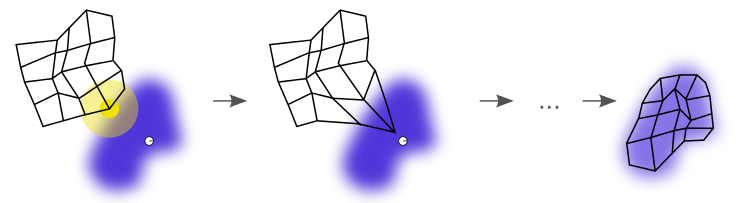
\includegraphics[width=0.6\linewidth]{fig/som1}
    \end{center}
    \caption{\textbf{SOM训练过程示意图.} 图来自wiki}
        \label{fig:plan}
  \end{figure}

\subsection{网络结构}

自组织神经网络本质上是一个两层的神经网络,包含输入层和输出层(竞争层). 输入层模拟感知外界输入信息的视网膜,输出层模拟做出响应的大脑皮层. 输入层的神经元数量由输入的维度决定, SOM网络结构的区别主要在竞争层: 可以有1维、2维(最常见的)

自组织映射的可见部分是映射空间(竞争层), 它由称为节点或神经元的单元组成。预先定义了映射空间,通常将其定义为有限的二维区域,其中节点以规则的六边形或矩形网格或排列, 见图\ref{fig:som2} 
\begin{figure}[h]
    \begin{center}
        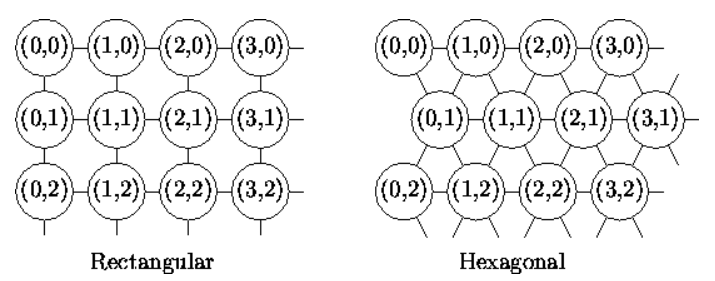
\includegraphics[width=0.6\linewidth]{fig/som2}
    \end{center}
    \caption{\textbf{SOM竞争层排列方式.} }
        \label{fig:som2}
  \end{figure}

在映射空间中, 每个神经元节点都与一个"权重"向量相关联, 该向量表征的是输入空间中的位置. 也就是说,神经元在数据结构上具有与每个输入向量(样本)相同的尺寸, 维度相同. 在映射空间中的节点保持固定的同时,训练包括将权重向量移向输入数据(减少距离度量, 而不会破坏从映射空间的拓扑。因此,自组织映射描述了从高维输入空间到低维映射空间的映射.
训练后, 该映射可以通过找到权重向量与输入空间向量最近(最小距离度量)最近的节点来对输入空间中的向量进行分类.%这句不明白

数人工神经网络一样,SOM以两种模式运行: 训练和映射. "训练"使用输入示例(竞争过程,也称为矢量量化)构建地图, 而"映射"自动分类新的输入矢量.

\subsection{网络训练}

网络训练的过程, 就是将输出层结点尽可能的扩张到训练集空间的过程, 其可以分为以下几个步骤:

\begin{itemize}
    \item[\textbf{0}] 初始化: 将神经元的权重初始化为较小的随机值,或者从两个最大主成分 特征向量跨越的子空间中均匀采样\footnote{使用后一种替代方法,学习速度要快得多,因为初始权重已经可以很好地近似SOM权重}.
    \item[\textbf{1}] 随机化: 随机取一个输入样本$X_i$,遍历竞争层中每一个结点, 计算$X_i$与节点之间的相似度(通常使用欧式距离)
    \item[\textbf{2}] 优胜神经元选择(Winner selection):取距离最小的节点作为优胜神经元节点 (winner node),有的时也叫BMU (best matching unit)
    \item[\textbf{3}] 近邻计算: 根据邻域半径$\sigma$确定优胜邻域将包含的节点,通过近邻函数计算它们各自更新的幅度, 基本思想是: 越靠近优胜节点,更新幅度越大.
    \item[\textbf{4}] 适应(Adaption):对所有竞争层神经元对应的权值进行更新, 一般使用Kohohen规则\cite{som}, 对解评估后, 返回第二步
\end{itemize}

现对网络训练关键的后三步进行详细描述:

\noindent{\textbf{优胜神经元选择(Winner selection)}}\\

优胜神经元(Best Match Unit)索引函数为:

\begin{eqnarray}
  \quad &j &=j(X_i)\\
  \nonumber
  \quad& &=\mathop{argmin}\limits_j \|X_i - W_j(n)\|, j=1, 2,\dots ,M
\end{eqnarray}
这里$M$为神经元的个数, $X_i$为随机选择的样本结点, $W_j$为$j$号神经元对应的权值向量,$n$为迭代步数.

\noindent{\textbf{近邻选择}}\\

近邻选择是一种加强中心, 抑制周围的神经元联结方式, 这是生物学竞争层中的一种天然近似. 一般情况下随着神经元之间的距离增加, 从加强到抑制的转变是平滑的出现的\cite{nnd2002}. SOM通过近邻函数来确定优胜节点(BMU)对其近邻节点的影响强弱,即优胜邻域中每个节点的更新幅度. 临近函数的输出维度与输出层神经元有着相同的拓扑结构, 其值对应着每个神经元你的变化幅度. 最常见的选择是高斯函数\footnote{也可以使用墨西哥草帽函数,Bubble函数等作为紧邻函数}, 它可以表征优胜邻域内, 影响强弱与距离的关系, 公式如下.

\begin{eqnarray}
  \quad & T(j,i,n) = e^{ - \frac{S^2(i,j)}{2\sigma^2(n)}},~~\sigma(n) = \sigma_0e^{- n  \verb|/| \tau}&
\end{eqnarray}
这里$S(j,i)$为衡量的为$j$号神经元与$i$号样本节点之间的距离,一般采用欧式距离; $\sigma$为邻域半径,初始值设为$\sigma_0 = 1$, $\tau$ 为一个接近1的小数, 我们这里设定$\tau = 0.99$.

\noindent{\textbf{适应(Adaptation))}}\\

适应过程就是权值向量的更新,根据上述两式子, 可以通过更新公式得到输出层权重的更新后的值:
\begin{eqnarray}
  \quad & W_j(n+1) = W_j(n)+ \alpha(n)\cdot T(j,i,n) \cdot|X_i - W_j(n)|&\\
  \nonumber
  \quad & \alpha(n) = \alpha_0e^{- n  \verb|/| \tau_\alpha}&
\end{eqnarray}
这里$\alpha_0 = 1 $, $\tau = 0.99$.




